\chapter{Références}

\begin{table}[!ht]
  \caption{Liste des options de compilations et leurs effets (non exhaustive), \url{https://gcc.gnu.org/onlinedocs/gcc/Optimize-Options.html}}
  \label{tab:compile_option}
  \small
  \begin{adjustwidth}{-2.1cm}{-2cm}
  \begin{center}
    \begin{tabular}{ll}
    \hlineB{2}
    \textbf{Option de compilation} & \textbf{Effet} \\
    \rowcolor{lightgray}
    -O0 & Compile le plus vite possible \\
    -O1 / -O & Compile en optimisant la taille et le temps d'exécution \\
    \rowcolor{lightgray}
    -O2 & Comme -O1 mais en plus fort, temps de compilation plus élevé mais exécution plus rapide\\
    -O3 & Comme -O2, avec encore plus d'options, optimisation du binaire\\
    \rowcolor{lightgray}
    -Os & Comme -O2 avec des options en plus, réduction de la taille du binaire au détriment du temps d'exécution  \\
    -Ofast & optimisations de la vitesse de compilation\\
    \rowcolor{lightgray}
    -Oz & optimisation agressive  sur la taille du binaire\\
    \hlineB{2}
    \end{tabular}
  \end{center}
  \end{adjustwidth}
\end{table}


\begin{figure}[!htb]
  \centering
  \begin{minipage}[b]{0.55\textwidth}
    \centering
    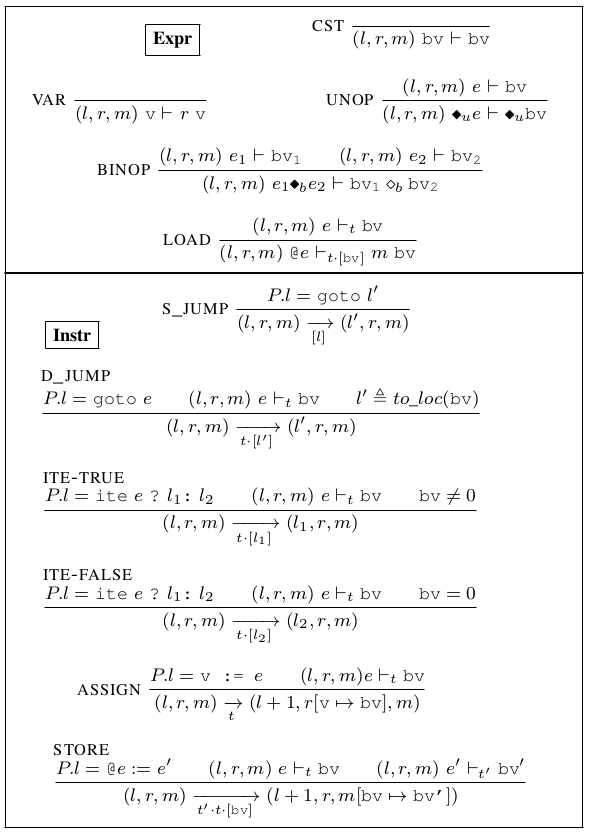
\includegraphics[scale=0.39]{pictures/instructions_formelles.png}
    \caption{Ensemble d'instructions défini formellement par \cite{binsecRel2019}}
    \label{fig:ensemble_instr_formelles}
  \end{minipage}\hfill
  \begin{minipage}[b]{0.4\textwidth}
    \textit{L'ensemble de ces règles a permis de décrire formellement le comportement
    de l'extension \texttt{checkct}, qui permet de vérifier les propriétés
    temps constants d'un programme.}
  \end{minipage}
\end{figure}


\chapter{Érysichthon, structure, exemples et résultats}

\begin{figure}[!ht]
  \centering
  
  \begin{tikzpicture}[scale= 1.3, transform shape]
    
    % Styles
    \tikzstyle{startstop} = [rectangle, rounded corners, minimum width=2cm, minimum height=1cm, text centered, draw=black, fill=green!30]
    \tikzstyle{process} = [rectangle, minimum width=2cm, minimum height=1cm, text centered, draw=black, fill=orange!30]
    \tikzstyle{arrow} = [thick,->,>=stealth]
    \tikzset{zone1/.style={rectangle, rounded corners, draw=red, dashed, fill=red!10, inner sep=0.3cm}}
    \tikzset{zone2/.style={rectangle, rounded corners, draw=blue, dashed, fill=blue!10, inner sep=0.5cm, text width=3cm}}
    \tikzset{zone3/.style={rectangle, rounded corners, draw=green, dashed, fill=green!10, inner sep=0.3cm}}
    \tikzset{zone4/.style={rectangle, rounded corners, draw=green, dashed, fill=green!30!blue!5, inner sep=0.3cm}}
    
    % Noeuds
    \node (make_test) [startstop] {ANDHRÍMNIR};
    \node (test) [below of = make_test] {Génère les tests};
    \node (test1) [below of=test, xshift=0.5cm, yshift=0.6cm] {\small{test1}};
    \node (test2) [below of=test1, yshift=0.6cm] {\small{test2}};
    \node (test3) [below of=test2, yshift=0.6cm] {\small{test3}};
    \node (test4) [below of=test3, yshift=0.6cm] {\small{test4}};
    \node (dots) [below of=test4, yshift=0.6cm] {\small{$\dots$}};
    
    \foreach \node in {test1, test2, test3, test4, dots} {
      \draw (test.south) |- (\node.west);
      }
      
    \node (start) [startstop, right of=make_test, yshift=2cm, xshift = 4cm] {Érysichthon};
    \node (blanc) [right of=make_test,yshift=-1cm, xshift = 2cm] {};
    \node (compilateur) [below of = start] {Compilateur};
    \node (hacl) [below of = compilateur, xshift=2cm] {Compile Hacl*};
    \node (tests) [below of = hacl, yshift = 0.3cm] {Compile les tests};
    \node (binsec) [below of = tests, xshift=1.8cm] {Exécute Binsec};
    \node (analyse) [below of = binsec, yshift = 0.3cm] {Étude des résultats};
    % Flèches
    \draw [arrow] (compilateur) |- (hacl.west);
    \draw [arrow] (compilateur) |- (tests.west);
    \draw [arrow] (tests) |- (binsec.west);
    \draw [arrow] (tests) |- (analyse.west);

    % Zones
    \begin{scope}[on background layer]
        \node (zone2node) [zone2, fit=(start) (compilateur) (hacl) (tests) (binsec) (analyse) (make_test) (test) (test1) (test2) (test3) (test4) (dots)] {};
        \node (title) [anchor=north west] at (zone2node.north west) {\parbox{3.5cm}{\centering \Huge{\textbf{Érysichthon}}\\\scriptsize{\textit{Panneau de contrôle}}}};
        \node (zone_tests) [zone1, fit=(make_test) (test) (test1) (test2) (test3) (test4) (dots)] {};
        \node (zone_compilation) [zone3, fit=(start) (compilateur) (hacl) (tests) (binsec) (analyse)] {};
        \node (zone_binsec) [zone4, fit=(binsec) (analyse)] {};
    \end{scope}

    % Flèches 2
    
    \draw [arrow, dashed, opacity=0.5] (title) -- (zone_tests);
    \draw [arrow, dashed, opacity=0.5] (title) -- (zone_compilation.west);
    \draw [thick,>=stealth, dashed, opacity=0.4] (title) -- (blanc.north);
    \draw [arrow, dashed, opacity=0.5] (blanc.north) -- (zone_binsec);
    \draw [arrow, dashed, opacity=0.2] (zone_tests.north) -- (zone_compilation.west);
  \end{tikzpicture}
  \caption{Structure d'Érysichthon, schéma du point de vue de l'usager}
  \label{fig:erysichthon_structure}
  \small
  Les flèches grises indiquent tous les éléments actionnables individuellement.
\end{figure}

\newpage
\begin{listing}[!ht]
  \caption{Déclaration de la fonction \textbf{encrypt} dans le fichier d'en-tête Hacl\_AEAD\_\-Chacha20Poly1305\_Simd256.h}
  \label{lst:exemple_header}
  \begin{minted}[
frame=lines,
framesep=2mm,
baselinestretch=1.2,
fontsize=\footnotesize,
linenos
]{c}
/**
Encrypt a message `input` with key `key`.

The arguments `key`, `nonce`, `data`, and `data_len` are same in encryption/decryption.
Note: Encryption and decryption can be executed in-place, i.e.,
`input` and `output` can point to the same memory.

@param output Pointer to `input_len` bytes of memory where the ciphertext is written to.
@param tag Pointer to 16 bytes of memory where the mac is written to.
@param input Pointer to `input_len` bytes of memory where the message is read from.
@param input_len Length of the message.
@param data Pointer to `data_len` bytes of memory where the associated data is read from.
@param data_len Length of the associated data.
@param key Pointer to 32 bytes of memory where the AEAD key is read from.
@param nonce Pointer to 12 bytes of memory where the AEAD nonce is read from.
*/
void
Hacl_AEAD_Chacha20Poly1305_Simd256_encrypt(
  uint8_t *output,
  uint8_t *tag,
  uint8_t *input,
  uint32_t input_len,
  uint8_t *data,
  uint32_t data_len,
  uint8_t *key,
  uint8_t *nonce
);
  \end{minted}
\end{listing}

\vfill
\begin{listing}[!htb]
  \caption{Extrait du fichier Hacl\_AEAD\_Chacha20Poly1305\_Simd256.json}
  \label{lst:exemple_json}
  \begin{minted}[
frame=lines,
framesep=2mm,
baselinestretch=1.2,
fontsize=\footnotesize,
linenos
]{json}
{
"Meta_data":{
    "build" : "13-06-2025",
    "version" : "0.2.0"
}

,"Hacl_AEAD_Chacha20Poly1305_Simd128_encrypt": {
    "*output":"BUF_SIZE"
   ,"*input":"BUF_SIZE"
   ,"input_len":"BUF_SIZE"
   ,"*data":"AAD_SIZE"
   ,"data_len":"AAD_SIZE"
   ,"*key":"KEY_SIZE"
   ,"*nonce":"NONCE_SIZE"
   ,"*tag":"TAG_SIZE"
   ,"BUF_SIZE":16384
   ,"TAG_SIZE":16
   ,"AAD_SIZE":12
   ,"KEY_SIZE":32
   ,"NONCE_SIZE":12
 }
}
  \end{minted}
\end{listing}

\newpage
\begin{listing}[!htb]
  \caption{Code généré du fichier test Hacl\_AEAD\_\-Chacha20\-Poly1305\_Simd256\_\-encrypt.c}
  \label{lst:exemple_complet}
  \begin{minted}[
frame=lines,
framesep=2mm,
baselinestretch=1.2,
fontsize=\footnotesize,
linenos
]{c}
//
// Made by
// ANDHRÍMNIR - 0.5.4
// 12-08-2025
//

#include <stdlib.h>
#include "Hacl_AEAD_Chacha20Poly1305_Simd128.h"

#define BUF_SIZE 16384
#define TAG_SIZE 16
#define AAD_SIZE 12
#define NONCE_SIZE 12
#define KEY_SIZE 32
uint8_t output[BUF_SIZE];
uint8_t tag[TAG_SIZE];
uint8_t input[BUF_SIZE];
uint32_t input_len_encrypt = BUF_SIZE;
uint8_t data[AAD_SIZE];
uint32_t data_len_encrypt = AAD_SIZE;
uint8_t key[KEY_SIZE];
uint8_t nonce[NONCE_SIZE];


int main (int argc, char *argv[]){
Hacl_AEAD_Chacha20Poly1305_Simd128_encrypt(output, tag, input, input_len_encrypt,
 data, data_len_encrypt, key, nonce);
   exit(0);
}
  \end{minted}
\end{listing}

\begin{listing}[!htb]
  \caption{Instruction Binsec générée automatiquement, \\ Hacl\_\-AEAD\_\-Chacha20Poly\-1305\_\-Simd256\_encrypt.ini}
  \label{list:exemple_ini_final}
  \begin{minted}[
frame=lines,
framesep=2mm,
baselinestretch=1.2,
fontsize=\footnotesize,
linenos
]{c}
starting from core

secret global output, input, data, key, nonce, tag
replace opcode 0f 01 d6 by
zf := true
end
replace opcode 0f 05 by
  if rax = 231 then
    print ascii "exit_group"
    print dec rdi
    halt
  end
  print ascii "syscall"
  print dec rax
  assert false
end
halt at <exit>    
  \end{minted}
\end{listing}


\newpage
\begin{table}[!th]
\centering
\begin{adjustwidth}{-20mm}{0mm}
\begin{minipage}{0.48\textwidth}
    \centering
    \begin{tabular}{c|ccc}
        \textbf{Optimisation} & \textbf{Secure} & \textbf{Unknown} & \textbf{Insecure} \\
        \hline
        \rowcolor{blue!5}
        -O0 & 359 & 168 & 21 \\
        -O1 & 372 & 154 & 22 \\
        \rowcolor{blue!5}
        -O2 & 378 & 148 & 22 \\
        -O3 & 382 & 139 & 27 \\
        \rowcolor{blue!5}
        -Os & 372 & 154 & 22 \\
        -Oz & 373 & 153 & 22 \\
    \end{tabular}
    \caption{Résultats d'Érysichthon en x86\_64}
    \label{tab:resultats_finaux}
\end{minipage}%
\hfill
\begin{minipage}{0.48\textwidth}
    \centering
    \begin{tabular}{c|cccccc}
        \textbf{Erreur / Option} & \textbf{-O0} & \textbf{-O1} & \textbf{-O2} & \textbf{-O3} & \textbf{-Os} & \textbf{-Oz} \\
        \hline
        \rowcolor{blue!5}
        KO        & 0  & 0  & 2  & 2  & 0  & 0  \\
        syscall   & 0  & 0  & 0  & 0  & 0  & 0  \\
        \rowcolor{blue!5}
        max depth & 92 & 59 & 45 & 23 & 58 & 59 \\
        killed    & 6  & 12 & 12 & 7  & 12 & 12 \\
        \rowcolor{blue!5}
        error     & 19 & 46 & 46 & 46 & 46 & 46 \\
        timeout   & 14 & 0  & 6  & 24 & 0  & 0  \\
        \rowcolor{blue!5}
        symbole    & 37 & 37 & 37 & 37 & 37 & 37 \\
    \end{tabular}
    \caption{Tableau détaillant les erreurs interrompant l'analyse Binsec}
    \label{table:detail_unknown}
\end{minipage}
\end{adjustwidth}
\end{table}


\raggedleft
\begin{table}[!ht]
  \begin{tabular}{l|cccccc}
    \textbf{Fonctions} & \multicolumn{6}{c}{\textbf{Options concernées}} \\
    \hline
    \rowcolor{blue!5}
    Hacl\_EC\_Ed25519\_point\_eq & O0 & O1 & O2 & O3 & Os & Oz \\
    Hacl\_K256\_ECDSA\_ecdh & O0 & O1 & O2 & O3 & Os & Oz \\
    \rowcolor{blue!5}
    Hacl\_K256\_ECDSA\_ecdsa\_verify\_hashed\_msg & O0 & O1 & O2 & O3 & Os & Oz \\
    Hacl\_K256\_ECDSA\_ecdsa\_verify\_sha256 & O0 & O1 & O2 & O3 & Os & Oz \\
    \rowcolor{blue!5}
    Hacl\_K256\_ECDSA\_is\_public\_key\_valid & O0 & O1 & O2 & O3 & Os & Oz \\
    Hacl\_K256\_ECDSA\_public\_key\_compressed\_from\_raw & O0 & & & & & \\
    \rowcolor{blue!5}
    Hacl\_K256\_ECDSA\_public\_key\_uncompressed\_to\_raw & O0 & O1 & O2 & O3 & Os & Oz \\
    Hacl\_K256\_ECDSA\_secp256k1\_ecdsa\_is\_signature\_normalized & O0 & O1 & O2 & O3 & Os & Oz \\
    \rowcolor{blue!5}
    Hacl\_K256\_ECDSA\_secp256k1\_ecdsa\_signature\_normalize & O0 & O1 & O2 & O3 & Os & Oz \\
    Hacl\_K256\_ECDSA\_secp256k1\_ecdsa\_verify\_hashed\_msg & O0 & O1 & O2 & O3 & Os & Oz \\
    \rowcolor{blue!5}
    Hacl\_K256\_ECDSA\_secp256k1\_ecdsa\_verify\_sha256 & O0 & O1 & O2 & O3 & Os & Oz \\
    Hacl\_NaCl\_crypto\_box\_open\_detached\_afternm & O0 & O1 & O2 & O3 & Os & Oz \\
    \rowcolor{blue!5}
    Hacl\_NaCl\_crypto\_secretbox\_open\_detached & O0 & O1 & O2 & O3 & Os & Oz \\
    Hacl\_P256\_compressed\_to\_raw & O0 & & & & &  \\
    \rowcolor{blue!5}
    Hacl\_P256\_dh\_responder & O0 & O1 & O2 & O3 & Os & Oz \\
    Hacl\_P256\_ecdsa\_verif\_p256\_sha2 & O0 & O1 & O2 & O3 & Os & Oz \\
    \rowcolor{blue!5}
    Hacl\_P256\_ecdsa\_verif\_p256\_sha384 & O0 & O1 & O2 & O3 & Os & Oz \\
    Hacl\_P256\_ecdsa\_verif\_p256\_sha512 & O0 & O1 & O2 & O3 & Os & Oz \\
    \rowcolor{blue!5}
    Hacl\_P256\_ecdsa\_verif\_without\_hash & O0 & O1 & O2 & O3 & Os & Oz \\
    Hacl\_P256\_uncompressed\_to\_raw & O0 & O1 & O2 & O3 & Os & Oz \\
    \rowcolor{blue!5}
    Hacl\_P256\_validate\_public\_key & O0 & O1 & O2 & O3 & Os & Oz \\
    Hacl\_FFDHE\_ffdhe\_shared\_secret\_precomp & & O1 & O2 & O3 & Os & Oz \\
    \rowcolor{blue!5}
    Hacl\_K256\_ECDSA\_secp256k1\_ecdsa\_sign\_hashed\_msg & & O1 & O2 & O3 & Os & Oz \\
    Hacl\_K256\_ECDSA\_secp256k1\_ecdsa\_sign\_sha256 & & O1 & O2 & O3 & Os & Oz \\
    \rowcolor{blue!5}
    Hacl\_NaCl\_crypto\_box\_beforenm & & & & O3 & &  \\
    Hacl\_NaCl\_crypto\_box\_detached & & & & O3 & &  \\
    \rowcolor{blue!5}
    Hacl\_NaCl\_crypto\_box\_easy& & & & O3 & &  \\
    Hacl\_NaCl\_crypto\_box\_open\_detached & & & & O3 & & \\
    \rowcolor{blue!5}
    Hacl\_NaCl\_crypto\_box\_open\_easy& & & & O3 & &  \\
  \end{tabular}
  \caption{Détails des fonctions non sécurisées en fonction des optimisations entrées, éxecution d'Érysichthon en x86\_64}
  \label{tab:resultats_insecure}
\end{table}
